%---------------------------------------------------------------------------------------------------
%		paas.tex
%
%	This is the main file of the chapter that talk about the paas layer of SPI.
%
%	Author: Andrea Meneghinello
% Version: 0.1
%	Table of changes:
%		15/03/2016 -> document definition
%---------------------------------------------------------------------------------------------------
\section{\acf{paas}}
\label{sec:problemSpace-paas}
\keyword{\ac{paas}} is like a \glossarySng{middleware}. It is a set of services that helps developers
to develop and test software without having to worry about provisioning servers, storage and backup
associated with developing and launching a new service. Developers want to write code, test the service,
launch it and be able to continually make changes to it to fix bugs. All the back-end issues about setting
up servers should be done automatically and transparently in background.

\ac{paas} and middleware are not the same thing. The main purpose of middleware is to offer
sophisticated features to developers, such as: transactions, security, clustering, etc. These features
allow them to build their custom applications instead of solving those hard problems repeatedly.
However middleware is only ``static'' software meaning that it must be configured, deployed and
administrated on servers by qualified personnel. All those tasks are usually assigned to \acs{it} teams.
Instead \ac{paas} is a superset of middleware and offers all these good features to developers
in addition to covering the operational aspects that where typically owned by \acs{it} teams.

Figure \ref{img:problemSpace-paas-spiResponsibilities} illustrates, in a transparent way, what are the
developers responsibility in the different stacks which compose the \ac{spi} model. We can see that
if we adopt the \ac{paas} model, we are only responsible for our code and its data.

\begin{figure}
	\centering{}
	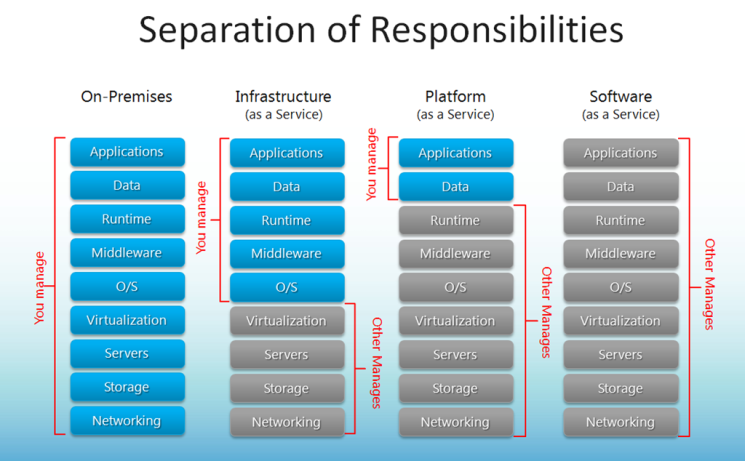
\includegraphics[width=0.8\textwidth]{chapters/problem/images/separation-responsabilities.png}
	\caption[Separation of responsability in \acs{spi}]{Separation of responsability in different stacks
		of the \acf{spi} model compared with the on premises one \cite{spiRepsonabilities}.}
	\label{img:problemSpace-paas-spiResponsibilities}
\end{figure}

As we argued in Section \ref{sec:problemSpace-cloudDepoymentModels}, \ac{paas} is possible because
is ``sitting'' over the \ac{iaas} infrastructure and through virtualization is able to provide many
features to developers. In following sections we will deep the concept of \ac{paas}
analysing its main characteristics and and the scenarios in which it is mostly useful. We will also
do a brief digression about virtualization, its main characteristics and available types.

\subsection{\acs{paas}: main characteristics}
\label{sec:problemSpace-paas-paasCharacteristics}
\ac{paas} offers to developers the following basic characteristics:

\begin{itemize}
	\item{it is able to maintain, inside the same \ac{ide}, services to develop, test and deploy
		applications;}
	\item{web based \ac{ui} creation tools help to create, modify, test and deploy different \ac{ui}
		scenarios;}
	\item{it makes possible multi-tenant architectures where multiple concurrent users utilize the same
		development application;}
	\begin{itemize}
		\item{support for development team collaboration: some \ac{paas} solutions can include project
			planning and communication tools;}
	\end{itemize}
	\item{it makes possible multi-tenant architectures where multiple concurrent users utilize the same
		deployed application\footnote{The application must be designed to support multiple concurrent
			users.};}
	\item{built in scalability of deployed software including load balancing and fault-tolerance;}
	\item{integration with databases and web services via common standards;}
	\item{tool to handle billing and subscription management.}
\end{itemize}

\ac{paas} is similar in many ways to \ac{iaas} but differentiate from it by the addition of value added
services and comes in two various types:

\begin{itemize}
	\item{a collaborative platform for software development, focused on workflow management regardless
		of the data source being used for the application. An example of this approach is Heroku, a
		\ac{paas} that utilizes Ruby on Rails language;}
	\item{a platform that allows for the creation of software that utilizing proprietary data from an
		application. This sort of \ac{paas} can be seen as a method to create applications with a common
		data form or type. An example is the Force.com from Salesforce.com which is used almost exclusively
		to develop applications that work with the Salesforce.com \ac{crm} tools.}
\end{itemize}

\ac{paas} owns the aforementioned characteristics because exploit better the feature that \ac{iaas}
is able to provide though virtualization. In the next section we will deep the concept of virtualization
to get to present the \acs{os} level of virtualization that cover a relevant part of this thesis.

\subsection{Virtualization}
\label{sec:problemSpace-paas-virtualization}
Both \ac{paas} and \ac{iaas} layer of \ac{spi} model are possible through virtualization techniques.
With the term \keyword{virtualization} we refer to the act of creating a virtual version of something,
including, but not limited, to a virtual computer hardware platform, \acs{os}es, storage devices or
network resources. Thus we can assert that virtualization is an isomorphism\footnote{Isomorphism is
a term that derive from the mathematics	domain and refers to a bijective application between objects
from different set.} between the virtual system, known as \keyword{guest}, and real one known as
\keyword{host}.

Through virtualization we want to provide high levels of performance and also gain in scalability,
reliability, availability and also in agility. Virtualization provides us an artificial view of the
physical world, on which many resources are viewed as single one or the opposite (one resource
is viewed as many individuals). Furthermore it can make a single large storage resource appear to be much
smaller or the opposite (many storage devices can appear as a big single device). It is also able to group
related processes together without making them able to see processes of other groups.

In this area virtualization provides a virtual version of a computer system, known with the name of
\keyword{\ac{vm}}. \citeauthor{vmArchitecture} in \cite{vmArchitecture} define \ac{vm} as:

\begin{quote}
	``a component that provides a complete, persistent system environment that support an \acs{os}
	along with its many users's processes. It provides the guest operating system which access to
	virtual hardware resources including networking, I/O, \ac{gui} along with processors and memory.''
\end{quote}

Virtualizing physical infrastructures helps to improve their scalability and their utilization. It is 
important to notice that it also enables the \acs{it} personnel to perform administration tasks in an
easier way. In the next section we will do a brief digression about the \ac{iaas} model and analyse
which assets are provided the other \ac{spi} models.

\subsubsection{Assets for cloud computing}
\label{sec:problemSpace-paas-virtualization-assets}
As we asserted in the precedent section, \ac{paas} is possible only because \ac{iaas} model exists.
To correctly support other \ac{spi} models it must provide them the following assets:

\begin{itemize}
	\item{\keyword{computing}: means executing users' tasks with the appropriate compute capacity. It is
		able to aggregate multiple computational resources to provide more power, or sharing the available
		resources in order to support tasks coming from different users. Anyway it must ensure
		\keyword{isolation}, \keyword{security} and \keyword{fast scalability};}
	\item{\keyword{storage}: means hiding physical storage devices, their location and their sharing between
		multiple users. Storage virtualization provides the following features: \ac{dfs},
		artificial storage volumes, arrays of storage volumes, a greater control over the available space and
		finally that different architecture can share the same storage devices;}
	\item{\keyword{networking}: means hiding the real complexity of the network by separating (or aggregating)
		the overall network system into manageable parts. Usually network virtualization provides the 
		following features: routing, \ac{nat}, isolation and aggregation.}
\end{itemize}

\subsubsection{Virtualization types}
\label{sec:problemSpace-paas-virtualization-types}
There exists two type of virtualization and they differ for the level in which they offer it; they
are: \keyword{hardware level virtualization} (virtualize over \ac{isa}) and \keyword{\acs{os} level
virtualization} (virtualize over \ac{abi} level). In this thesis we are mostly interested in \acs{os}
level virtualization; Further analysis about the first one can be found in \citeauthor{gardimanThesis}'s
master thesis \cite{gardimanThesis}.
Figure \ref{img:problemSpace-paas-virtualization-assets-virtualizationLevels}
shows a generic computer architecture and highlights the possible level of virtualization.

\begin{figure}
	\centering{}
	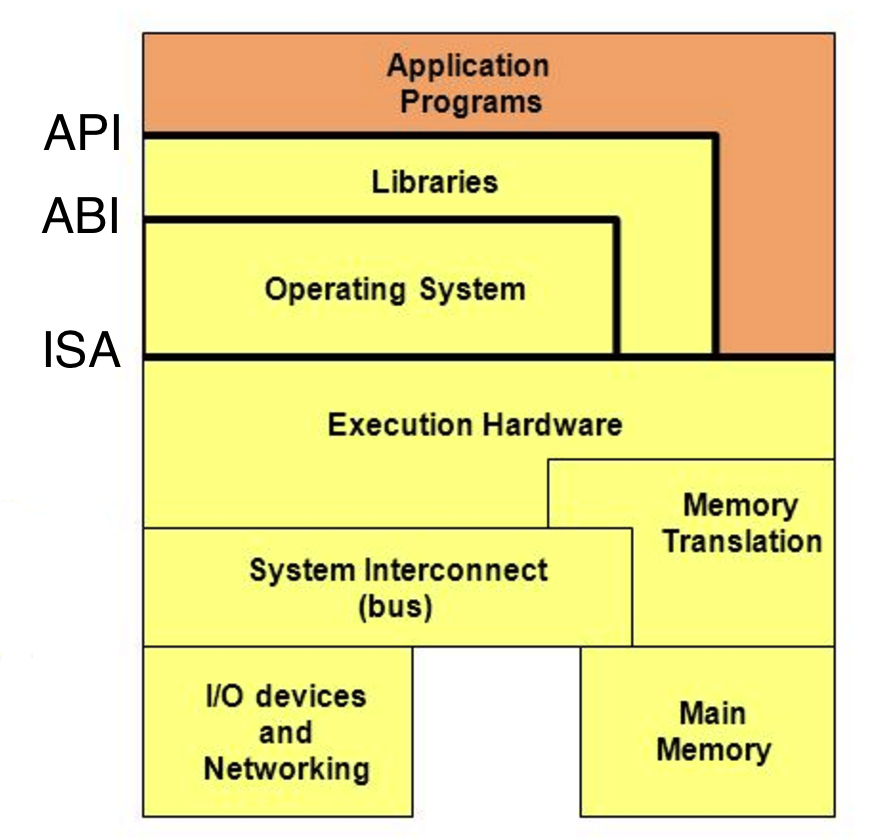
\includegraphics[width=0.5\textwidth]{chapters/problem/images/computing-virtualization.png}
	\caption[Different computing virtualization levels]{Overview of computer architecture that shows at
		which layer we can provide virtualization. \acf{iaas} allow virtualization over \acf{isa}, instead
		\ac{paas} provide virtualization over \acf{abi} and finally \ac{saas} allows virtualization over
		\ac{api} \cite{virtualizationLevel}.}
	\label{img:problemSpace-paas-virtualization-assets-virtualizationLevels}
\end{figure}

To be thorough, we are going to spend some words about hardware level virtualization in order to correctly
understand the difference with the other type. At Hardware level the virtualization isomorphism is managed
by a software layer called \keyword{hypervisor}, which can be of two different types (shown in Figure 
\ref{img:problemSpace-paas-virtualization-assets-virtualizationTypes}):

\begin{itemize}
	\item{\keyword{native} (type 1): a native hypervisor runs directly over the physical hardware ensuring
		a complete control of the same. In this case the hypervisor must be compatible with all the physical
		hardware thus being able to manage it;}
	\item{\keyword{hosted} (type 2): a hosted hypervisor runs over an host \acs{os} which lies above the
		physical architecture; this topology delegates to the host \acs{os} the following tasks: hardware
		drivers management, available memory management, resources allocation management and finally process
		scheduling.}
\end{itemize}

The hosted hypervisor can produce a reduction of the perceived performance because of the presence of a 
further layer that the native type does not have. As a consequence a system, call originated by an 
application or service inside one \ac{vm}, needs more time to reach the underlying hardware downgrading 
the general performance.

\begin{figure}
	\centering{}
	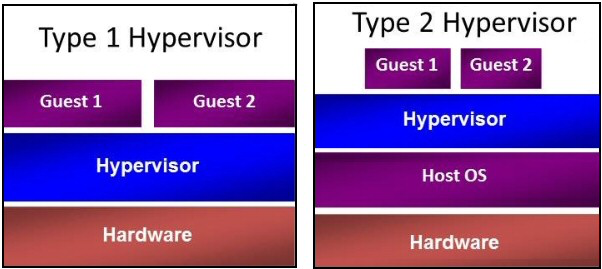
\includegraphics[width=0.6\textwidth]{chapters/problem/images/virtualization-types.png}
	\caption[Virtualization types]{The stack generated by the two different type of virtualization.
		We can see the native (type 1) on the left and hosted one (type 2) on the right
		\cite{virtualizationTypes}.}
	\label{img:problemSpace-paas-virtualization-assets-virtualizationTypes}
\end{figure}

The hypervisor can virtualize the underlying hardware using three different approaches:

\begin{itemize}
	\item{\keyword{full-virtualization}: the hypervisor completely virtualizes the underlying hardware,
		ensuring a full compatibility with any \acs{os} that supports the physical infrastructure;}
	\item{\keyword{hardware-assisted virtualization}: the hypervisor is built as an extension of the
		previous one (full-virtualization). In this case the processor has a built-in architectural support
		that facilitate the forward phase, to the underlying hardware, of a system call generated by an
		application or service that runs inside a \ac{vm};}
	\item{\keyword{para-virtualization}: hypervisor does not offer an interface that simulates the
		underlying hardware but exposes a modified one to \ac{vm}s (closer the real one), called Virtual
		Hardware \acs{api}, explicitly designed for the \ac{vm}s; an advantage of this type of virtualization
		is that it is possible to implement an interface agnostic to the underlying hardware; instead
		the major weakness is that in case of a system crash all the current \ac{vm}s will be affected by
		the problem.}
\end{itemize}

Unlike hardware level virtualization, \acs{os}-virtualization  provides a virtual view over the
\ac{abi}. In this case the guest and the host share same \acs{os} and host hardware.

Users' processes execute on the host and they are (as much as possible) isolated from each other.
Logical separated environments are called \keyword{containers}.
Figure \ref{img:problemSpace-paas-virtualization-assets-virtualizationTypeDifference} shows the
difference between \acs{os} level virtualization and hardware level one.

\begin{figure}
	\centering{}
	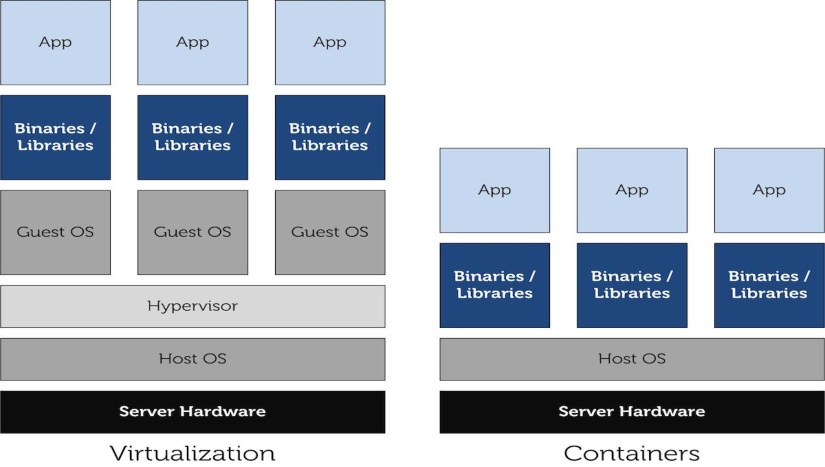
\includegraphics[width=0.7\textwidth]{chapters/problem/images/containerization.png}
	\caption[Difference from containerization and virtualization]{Difference from the generated stack
		by hardware level virtualization (type 2) and containerization.}
	\label{img:problemSpace-paas-virtualization-assets-virtualizationTypeDifference}
\end{figure}

Containers technology has existed for a long time. Examples of containers that runs outside Linux
ecosystem are Solaris Zones \cite{solarisContainers}, and \acs{bsd} jails \cite{bsdContainers}.
Instead containers' technology for the Linux ecosystem are: Linux-Vserver \cite{vserverContainers}
and OpenVZ \cite{openvzContainers}. Even though all these technologies have matured, they did not make
significant progress in order to create a proper standard technology.

The containers landscape changed when Linux containers reached a level of maturity that lead them 
into the mainstream Linux kernel with the project \keyword{\ac{lxc}}. This last one uses mainly two
kind of Linux kernel features: \keyword{namespaces} and \keyword{cgroups}.

The namespace is able to isolate processes resources though the following namespaces:

\begin{itemize}
	\item{PID: processes residing in a namespace cannot affect others namespace's processes. This
		means that processes inside a container are not able to see or alter processes that reside in
		another container;}
	\item{NET: each net-namespace have a different, and isolated view of the network interfaces. Each
		one has its own routing-table, iptable chains and rules;}
	\item{IPC: each process can communicate only with processes that are in the same \ac{ipc} group. This
		is necessary to maintain process isolation;}
	\item{MNT: processes that live in different mnt-namespace can see other sets of mounted \ac{fs} and
		root directories. If a \ac{fs} is mounted in an mnt-namespace, it will be accessible only to those
		that are in the same namespace;}
	\item{UTS: it is able to give containers a different host-name.}
\end{itemize}

Instead cgroups is able, through a set of rules, to measure and limit the resource consumption on which
containers have access.

\ac{lxc} is a good technology that allows users to run several applications isolated from each other. It
is able to assure an amount of resource capacity to each container. However, even with this feature,
Linux containers have never reached a wide level of adoption because of their lack in handiness. Everything
has changed when a company named ``docCloud'' delivered an open-source project called \keyword{Docker}.
We will deep about Docker and its architecture in Section \ref{sec:problemSpace-docker}.

\subsubsection{Main characteristics}
\label{sec:problemSpace-paas-virtualization-characteristics}
Virtualization has three main characteristics: partitioning, isolation and encapsulation.

\keyword{Partitioning} refers to the fact that many applications and \acs{os}es are supported in a single 
physical system by separating (partitioning) the available resources. \keyword{Isolation} refers to the
fact that each \ac{vm} is isolated from its physical system and other \ac{vm}; because of isolation, if
one virtual instance crashes it does not affect the others\footnote{Except in case of para-virtualization.}
and data are not shared between different \ac{vm}s\footnote{If data sharing between \ac{vm}s is a requirement
it must be implemented as a software feature.}. Finally \keyword{encapsulation} property derives from
the fact that \ac{vm}s are represented (and even stored) as a single file, hence system administrators
can identify them easily based on the service that they provide.

From the cited properties we can affirm that cloud computing and Virtualization are not interchangeable
because they approach the \acs{it} goals from different perspectives: virtualization has the aim to
isolate computing resources in order to make possible the change of underlying layers without worrying
about higher levels; instead cloud computing has the ability to make computing resources available on
demand providing us the pay-per-use paradigm.

\subsection{\acs{paas}: where to use}
\label{sec:problemSpace-paas-whereToUse}
\ac{paas} is very useful in any situation where multiple developers work on a development project or
where other external parties need to interact with the development process. As the case study illustrated
below, it is proving invaluable for those who have an existing data source, for example sales information
from a \ac{crm} tool, and want to create applications which leverage that data. Finally \ac{paas} is useful
where developers wish to automate testing and deployment services.

The popularity of \glossarySng{agile} will also increase the uptake of \ac{paas} as it eases the
difficulties around rapid development and iteration of software.

Some examples of \ac{paas} include \ac{gae} \cite{googleAppEngine}, Microsoft Windows Azure
\cite{windowsAzure} and finally Salesforce.com \cite{salesforcePlatform}.

\subsection{\acs{paas}: where do not to use}
\label{sec:problemSpace-paas-whereNotToUse}
There are many positive aspects that bring us adopting \ac{paas}, but there also some scenarios where it
may not be ideal. Examples include:

\begin{itemize}
	\item{where the applications need to be highly portable\footnote{In terms of where they are hosted.};}
	\item{where proprietary languages or approaches would impact on the development process;}
	\item{where a proprietary language would hinder later moves to others provides. Concerns are raised
		about vendor lock-in \cite{vendorLockin};}
	\item{where application performance requires customization of the underlying hardware and/or software.}
\end{itemize}

\subsection{\acs{paas}: a case study}
\label{sec:problemSpace-paas-caseStudy}
Menumate \cite{menumateCaseStudy} is a provider of point of sale hardware and software for the hospitality
industry across Australasia. It has taken advantage of the Force.com \ac{paas} to migrate over time a
series of legacy applications used in the business.

Trineo's \cite{trineoCaseStudy} directors of development explained that the use of Force.com platform has
allowed Menumate to centralise, modernise and integrate an otherwise disparate in-house software toolkit. 
They also asserted that a more conventional development approach would require significant infrastructure,
connectivity, security; this also would introduce uptime considerations. Instead the Force.com
platform inherently provides these non-functional requirements, allowing both Menumate and Trineo to
focus purely on developing the needed functionality. Additionally, utilizing a \ac{paas} approach
has meant Trineo could take advantage of both existing integration and deployment tools.

Utilizing a \ac{paas} development environment has resulted in the creation of applications being
significantly faster than would otherwise be the case. In absence of \ac{paas}, the cost of developing
applications would be prohibitive for many companies.